许多现代编程语言都支持使用类面向对象方式。类是一种高级语言构造,在本节中,我们将探讨如何将类构造映射到LLVM IR中。\par

\hspace*{\fill} \par %插入空行
\textbf{实现单继承}

类是数据和方法的集合。一个类可以从另一个类继承,可能会添加更多的数据字段和方法,或者覆盖现有的虚方法。我们用Oberon-2中的类来说明这一点,它也是tinylang的一个模型。Shape类定义了一个带有颜色和区域的抽象形状:\par

\begin{tcolorbox}[colback=white,colframe=black]
TYPE Shape = RECORD \\
\hspace*{3cm}color: INTEGER; \\
\hspace*{3cm}PROCEDURE (VAR s: Shape)  GetColor(): \\
\hspace*{3.5cm}INTEGER; \\
\hspace*{3cm}PROCEDURE (VAR s: Shape) Area(): REAL;\\
\hspace*{2.5cm}END;
\end{tcolorbox}

GetColor方法只返回颜色编号:\par

\begin{tcolorbox}[colback=white,colframe=black]
PROCEDURE (VAR s: Shape) GetColor(): INTEGER; \\
BEGIN RETURN s.color; END GetColor;
\end{tcolorbox}

抽象的形状的面积是无法计算的,所以这是一个抽象方法:\par

\begin{tcolorbox}[colback=white,colframe=black]
PROCEDURE (VAR s: Shape) Area(): REAL; \\
BEGIN HALT; END;
\end{tcolorbox}

Shape类型可以扩展为表示Circle类:\par

\begin{tcolorbox}[colback=white,colframe=black]
TYPE Circle = RECORD (Shape) \\
\hspace*{3cm}radius: REAL; \\
\hspace*{3cm}PROCEDURE (VAR s: Circle) Area(): REAL; \\
\hspace*{2.5cm}END;
\end{tcolorbox}

对于圆,面积公式为:\par

\begin{tcolorbox}[colback=white,colframe=black]
PROCEDURE (VAR s: Circle) Area(): REAL; \\
BEGIN RETURN 2 * radius * radius; END;
\end{tcolorbox}

还可以在运行时查询该类型。如果shape是Shape类型的变量,则可以这样制定类型测试:\par

\begin{tcolorbox}[colback=white,colframe=black]
IF shape IS Circle THEN (* … *) END;
\end{tcolorbox}

除了语法不同之外,工作原理与C++非常相似。与C++的明显区别是,Oberon-2语法使隐式的this指针显式化,将其称为接收方方法。\par

需要解决的基本问题是如何在内存中布局类,以及如何实现方法的动态调用和运行时类型检查。对于内存布局,这是相当容易的。Shape类只有一个数据成员,可以将它映射到相应的LLVM结构类型:\par

\begin{tcolorbox}[colback=white,colframe=black]
@Shape = type \{ i64 \}
\end{tcolorbox}

Circle类添加了另一个数据成员,直接在末尾添加新的数据成员:\par

\begin{tcolorbox}[colback=white,colframe=black]
@Circle = type \{ i64, float \}
\end{tcolorbox}

原因是一个类可以有很多子类。使用这种策略,公共基类的数据成员总是具有相同的内存偏移量,并使用相同的索引通过getelementptr指令访问字段。\par

为了实现方法的动态调用,必须进一步扩展LLVM结构。如果在Shape对象上调用Area()函数,则会调用抽象方法,导致应用程序停止。如果在Circle对象上调用该函数,则调用相应的方法来计算圆的面积。这两个类的对象都可以调用GetColor()函数。实现这个的基本思想是将表与函数指针与每个对象关联起来。这里,该表有两个条目:一个用于GetColor()方法,一个用于Area()函数。Shape类和Circle类都有这样一个表。这两个表在Area()函数的条目上有所不同,该函数根据对象的类型调用不同的代码。这个表称为虚方法表,通常缩写为vtable。\par

单独使用vtable是没有用的,我们必须把它和一个物体联系起来。为此,可以添加一个指向虚函数表的指针,该指针总是作为结构的第一个数据成员。在LLVM层,@Shape类型变成如下表示:\par

\begin{tcolorbox}[colback=white,colframe=black]
@Shape = type \{ [2 x i8*]*, i64 \}
\end{tcolorbox}

@Circle类型的扩展也是类似的,得到的内存结构如图6.1所示:\par

\hspace*{\fill} \par %插入空行
\begin{center}
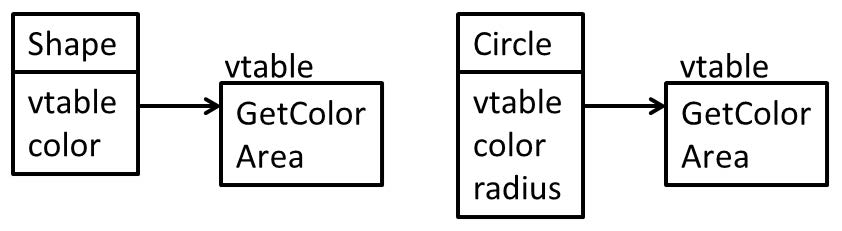
\includegraphics{content/2/chapter6/images/1.jpg}\\
图6.1 – 类和虚拟方法表的内存布局
\end{center}

LLVM没有空指针,而是使用指向字节的指针。引入了隐藏的虚函数表字段后,现在还需要一种方法来初始化它。在C++中,这是构造函数的一部分。在Oberon-2中,该字段在分配内存时自动初始化。\par

然后按以下步骤执行对方法的动态调用:\par

\begin{enumerate}
\item 通过getelementptr指令计算虚表指针的偏移量。
\item 加载指向虚函数表的指针。
\item 计算虚函数表中函数的偏移量。
\item 加载函数指针。
\item 通过带有调用指令的指针间接调用函数。
\end{enumerate}

这听起来不是很高效,但事实上,大多数CPU架构只需要两条指令就可以执行这个动态调用。因此,真正低效的是LLVM层。\par

要将函数转换为方法,需要对对象数据的引用。这是通过将指向数据的指针,作为函数的第一个参数来实现的。在Oberon-2中,这就是显式接收器。类似于C++的语言中的this指针。\par

有了虚函数表,每个类在内存中都有唯一的地址。这对运行时类型测试有帮助吗?的确有帮助,但帮助有限。为了说明这个问题,我们用继承自Circle类的Ellipse类来扩展类层次结构(这不是数学意义上的is-a关系)。如果有Shape类型的shape变量,那么可以实现shape IS Circle的类型测试,将shape变量中存储的虚函数表指针与Circle类中的虚函数表指针进行比较。只有当shape具有精确的Circle类型时,这个比较才会得到true。但是如果shape是Ellipse类型的,那么将返回false(即使Ellipse类型的对象,可以在只需要Circle类型的对象的地方使用)。\par

显然,我们需要做得更多。解决方案是使用运行时类型信息扩展虚拟函数表,需要存储多少信息取决于源语言。为了支持运行时类型检查,只要存储一个指向基类的虚函数表的指针就足够了,如图6.2所示:\par

\hspace*{\fill} \par %插入空行
\begin{center}
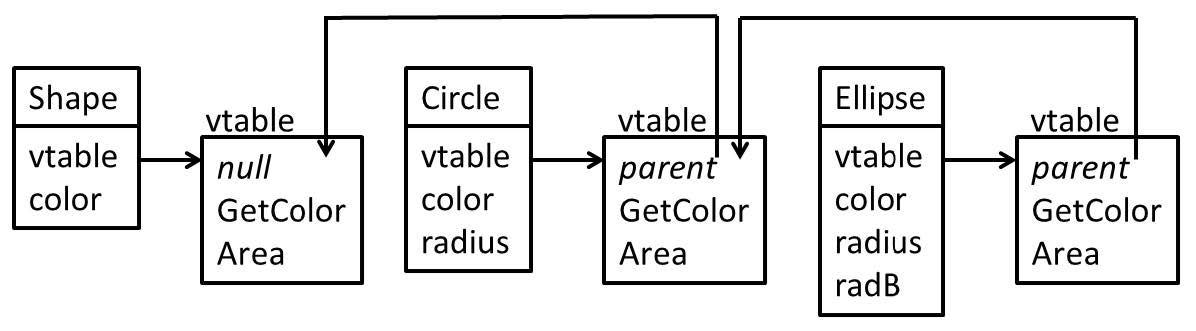
\includegraphics{content/2/chapter6/images/2.jpg}\\
图6.2 – 支持简单类型测试的类和虚函数表布局
\end{center}

若测试像前面描述的那样失败,则使用指向基类的虚函数表的指针重复测试。一直重复,直到测试结果为true,如果没有基类,则为false。与调用动态函数相比,类型测试是一种开销很大的操作,因为在最坏的情况下,继承层次结构会逐步上升到根类。\par

如果您知道整个类层次结构,那么就可能有一种有效的方法:按照深度优先的顺序为类层次结构的每个成员编号。然后,类型测试就变成了对一个数字或一个区间的比较,可以在固定时间内完成。事实上,这就是LLVM自己的运行时类型测试的方法,我们在前一章已经学习过了。\par

将运行时类型信息与虚函数表耦合是一个设计上的决策,要么由源语言强制执行,要么只是一个实现。如果您需要详细的运行时类型信息,因为源语言支持运行时反射,而您的数据类型没有虚函数表,那么耦合两者就不是一个好主意。在C++中,这种耦合出现在一种情况下,即带有虚函数(因此没有虚函数表)的类没有附加运行时类型数据。\par

编程语言通常支持接口,接口是虚拟方法的集合。接口很重要,它们添加了有用的抽象。我们将在下一节中讨论接口的可能实现。\par

\hspace*{\fill} \par %插入空行
\textbf{使用接口扩展单继承}

像Java这样的语言支持接口。接口是抽象方法的集合,类似于没有数据成员且只定义抽象方法的基类。接口带来了一个有趣的问题,因为每个实现接口的类在虚函数表的不同位置都有相应的方法。原因很简单,虚函数表中函数指针的顺序派生自源语言中类定义中函数的顺序。接口中的定义与此无关,不同的顺序才是重点。\par

因为在接口中定义的方法可以有不同的顺序,所以将每个实现的接口的表附加到类中。对于接口的每个方法,该表既可以指定方法在虚表中的索引,也可以指定存储在虚表中的函数指针的副本。如果在接口上调用方法,则搜索接口对应的虚函数表,然后获取函数的指针并调用方法。将两个接口I1和I2添加到Shape类中会得到如下布局:\par

\hspace*{\fill} \par %插入空行
\begin{center}
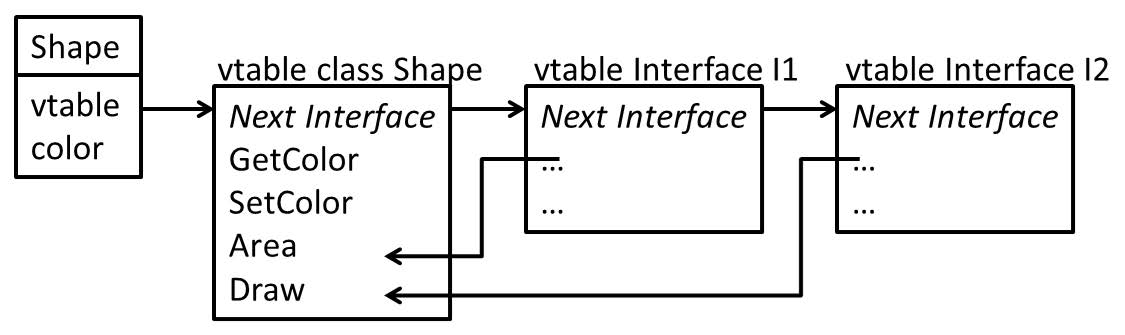
\includegraphics{content/2/chapter6/images/3.jpg}\\
图6.3 – 接口的虚函数表布局
\end{center}

需要注意的是,我们必须找到正确的虚变量表。可以使用类似于运行时类型测试的方法:可以通过接口虚函数表列表执行线性搜索。使用这个数字标识虚函数表,可以为每个接口分配一个唯一的数字(例如,内存地址)。这种模式的缺点很明显:通过接口调用方法要比在类上调用相同的方法花费更多的时间。要解决这个问题并不容易。\par

一个好的方法是用哈希表代替线性搜索。在编译时,类实现的接口已知。因此,可以构造一个哈希函数,它将接口编号映射到接口的虚函数表。在构造过程中可能需要一个已知标识接口的数字,因此内存没有帮助。但还有其他计算唯一数字的方法。如果源中的符号名是唯一的,那么可以计算加密哈希值,如符号的MD5,并使用哈希值作为数字。计算发生在编译时,因此没有运行时成本。\par

结果比线性搜索快得多,只需要常数时间。尽管如此,仍然涉及对数字的几个算术运算,比类类型的方法调用要慢。\par

通常,接口也会参与运行时类型测试,这使得需要搜索的列表更长。当然,如果实现了哈希表方法,那么它也可以用于运行时类型测试。\par

有些语言允许有多个父类。这对实现有一些挑战,我们将在下一节学习。\par

\hspace*{\fill} \par %插入空行
\textbf{对多重继承的支持}

多重继承增加了另一个挑战。如果一个类继承了两个或更多的基类,那么我们需要组合数据成员,使它们仍然可以从函数中访问。与单继承的情况一样,解决方案是附加所有数据成员,包括隐藏的虚函数表指针。Circle类不仅是一个几何形状,也是一个图形对象。为了对此进行建模,让Circle类继承Shape类和GraphicObj类。在类布局中,来自Shape类的字段最先出现。然后,附加GraphicObj类的所有字段,包括隐藏的虚表指针。之后,添加了Circle类的新数据成员,得到了如图6.4所示的整体结构:\par

\hspace*{\fill} \par %插入空行
\begin{center}
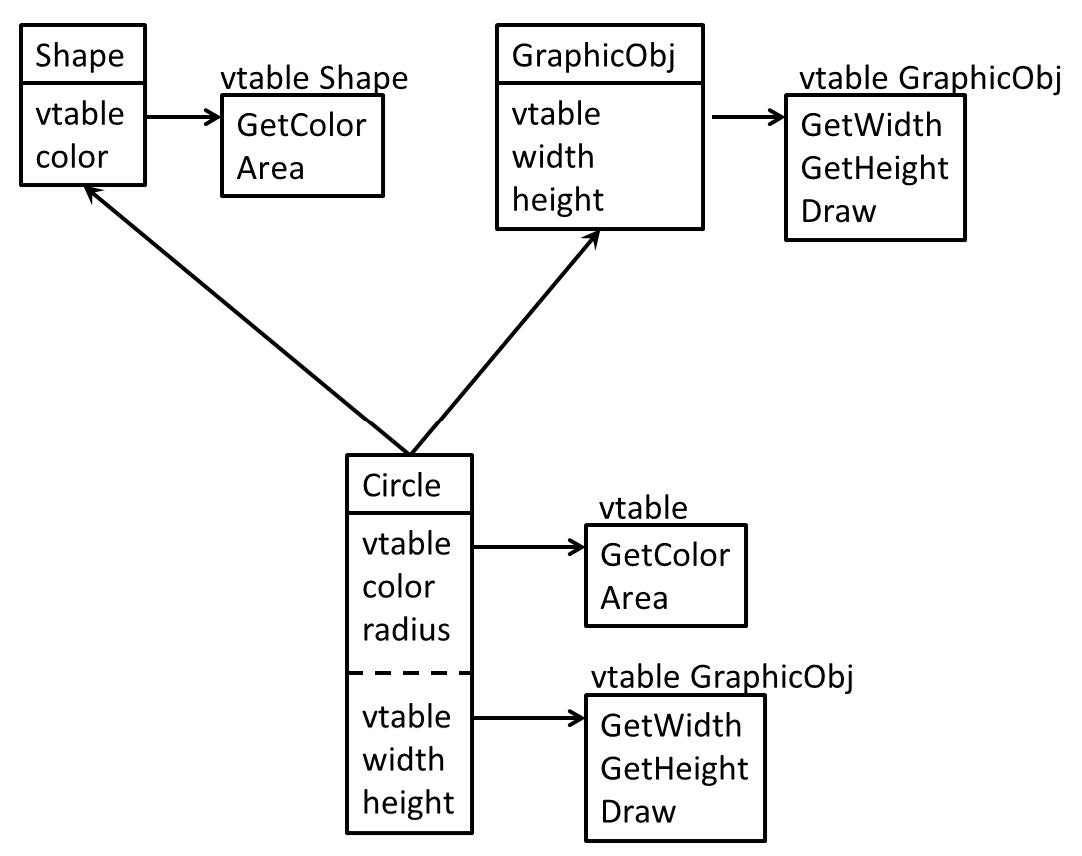
\includegraphics{content/2/chapter6/images/4.jpg}\\
图6.4 – 具有多重继承的类和虚函数表
\end{center}

这种函数有几个含义。现在可以有几个指向该对象的指针。指向Shape或Circle类的指针指向对象的顶部,而指向GraphicObj类的指针指向对象内部,指向嵌入的GraphicObj对象的开头。在比较指针时必须考虑这一点。\par

调用虚函数也会受到影响。如果函数是在GraphicObj类中定义的,那么这个函数需要GraphicObj类的类布局。如果这个函数没有在Circle类中重写,那么有两种可能。简单的情况是,如果函数调用是通过一个指向GraphicObj实例的指针完成的:在GraphicObj类的虚表中查找方法的地址,然后调用函数。更复杂的情况是使用指向Circle类的指针调用函数。同样,可以在Circle类的虚表中查找函数的地址。调用的函数需要一个指向GraphicObj类实例的this指针,因此我们也必须调整该指针。我们可以这样做,因为已知GraphicObj类在Circle类中的偏移量。\par

如果在Circle类中重写了GrapicObj的函数,通过指向Circle类的指针调用该方法,则不需要做任何特殊操作。但是,如果该方法是通过指向GraphicObj实例的指针调用的,就需要进行另一个调整,因为该方法需要一个this指针指向Circle实例。编译时,我们无法计算这个调整,因为不知道这个GraphicObj实例是否是多重继承层次结构的一部分。为了解决这个问题,我们将在调用函数之前对this指针所做的调整与虚函数表中的每个函数指针一起存储起来,如图6.5所示:\par

\hspace*{\fill} \par %插入空行
\begin{center}
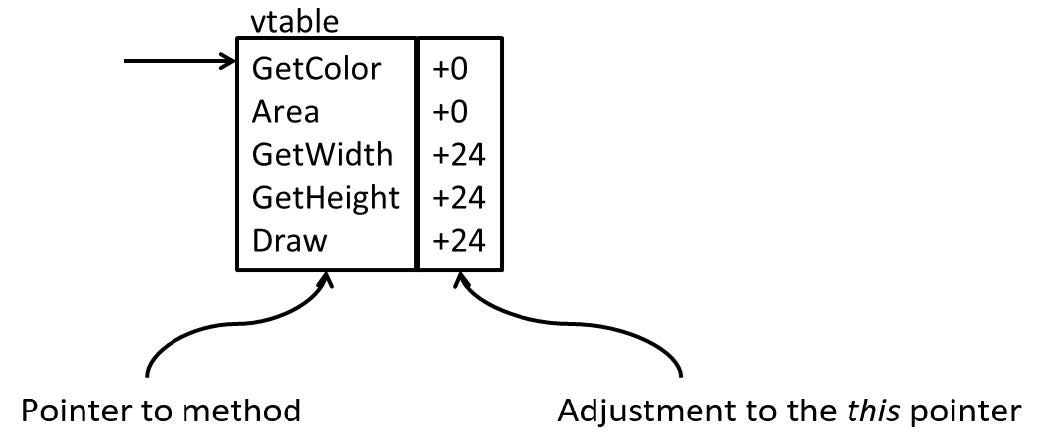
\includegraphics{content/2/chapter6/images/5.jpg}\\
图6.5 – 调整this指针的虚函数表
\end{center}

函数调用现在变成如下方式:\par

\begin{enumerate}
\item 在虚函数表中查找函数指针。
\item 调整this指针。
\item 调用该方法。
\end{enumerate}

这种方法还可以用于实现接口。因为接口只有方法,所以每个实现的接口都会向对象添加一个新的虚函数表指针。这更容易实现,而且可能更快,但它增加了每个对象实例的开销。在最坏的情况下,如果你的类有一个64位数据字段,实现了10个接口,那么你的对象需要96个字节的内存:类本身的vtable指针需要8个字节,数据成员需要8个字节,每个接口的vtable指针需要10 * 8个字节。\par

为了支持对对象的有意义的比较并执行运行时类型测试,需要首先对对象的指针进行标准化。如果我们在虚表中添加一个额外的字段,在对象的顶部包含一个偏移量,那么我们总是可以调整指针指向实际对象。在Circle类的虚函数表中,这个偏移量是0,但在嵌入式GraphicObj类的虚函数表中不是。当然,这是否需要实现取决于源语言的语义。\par

LLVM本身并不支持面向对象特性的特殊实现。如本节所见,可以使用可用的LLVM数据类型实现所有方法。如果想尝试一种新的方法,那么一个好方法是先用C做一个原型。所需的指针操作可以快速地转换为LLVM IR,但是在高级语言中进行功能性的推理会更容易。\par

通过本节,您可以在自己的代码生成器中将编程语言中所有OOP构造下沉至LLVM IR中。您已经了解了如何表示单继承、使用接口的单继承或内存中的多继承,以及如何实现类型测试和如何查找虚函数的方法,这些都是OOP语言的核心概念。\par





















